\documentclass[final,nopreprintline]{elsarticle}

\usepackage[colorlinks,allcolors=blue]{hyperref}
\usepackage{doi}
\usepackage{amssymb}
\usepackage{amsmath}
\usepackage{amsthm}
\usepackage{pdfpages}
\usepackage{lscape}
\usepackage{float}
\usepackage{multirow}
\usepackage[ngerman,american]{babel}  % für Silbentrennung
\usepackage{bibgerm}
\usepackage[symbol]{footmisc}
\renewcommand{\thefootnote}{\fnsymbol{footnote}}


\journal{Visual Analytics}
\begin{document}
\begin{frontmatter}

\title{Balancing Performance and Visual Appeal in Dynamic Graph Labeling}
\author{Nils Henrik Seitz\footnote[1]{\href{mailto:ns464@uni-rostock.de}{ns464@uni-rostock.de}} (Mat.Nr. 218205308)}
\address{Faculty of Computer Science \\University of Rostock}


\begin{abstract}
    Lörem ipsum dolör sit ämet, conßectetur adipiscing elit, sed do eiusmod tempor incididunt ut labore et dolore magna aliqua. Ut enim ad minim veniam, quis nostrud exercitation ullamco laboris nisi ut aliquip ex ea commodo consequat. Duis aute irure dolor in reprehenderit in voluptate velit esse cillum dolore eu fugiat nulla pariatur. Excepteur sint occaecat cupidatat non proident, sunt in culpa qui officia deserunt mollit anim id est laborum.

\end{abstract}


\end{frontmatter}


\textbf{Bemerkung:} Dieses Projekt wurde in Kooperation mit Nico Trebbin erstellt. Der Bericht wurde als eigenständiges Werk von dem Autor angefertigt.
Bilddateien haben gegebenenfalls einen gemeinsamen Ursprung als Material für die Präsentation im Rahmen des Projektes.

Viele der Kernbegriffe des Projektes werden in diesem Bericht im Original verwendet, um Konsistenz mit der Codebasis und den Präsentationen des Projektes zu erhalten.

\section{Einleitung}
\label{sec:intro}
    Graphen sind wohl die mit am meisten genutzte Datenstruktur der Informatik.
Durch sie lassen sich viele verschiedene Sachverhalte modellieren.
Mit \texttt{iGraph.js} existiert als praktische Grundlage ein Tool zur interaktiven und dynamischen Visualisierung von Graphen.

Das Problem ist, dass ohne die Namen der Knoten und Kanten dem Graph recht wenig Bedeutung abgewonnen werden kann,
es fehlt Kontext. Der Kontext kann durch ein Labeling des Graphen klarer werden. Dazu sind allerdings zwei Dinge zentral:

Erstens sollte das Labeling muss visuell ansprechend sein, das heißt, es muss intuitiv klar sein, welches Label zu welchem Knoten oder zu welcher Kante gehört
und es sollten keine Überdeckungen entstehen.

Zweitens sollte das Labeling performant sein, da selbst die schönste Anordnung von Labels nicht nützlich ist in einem dynamischen und interaktiven Umfeld, wenn sie zu lange zum Errechnen braucht.
Den bestmöglichen Kompromiss aus Labeling Qualität und Performance zu finden, ist die Kernaufgabe dieses Projektes.

Dazu haben wir eine Labeling Pipeline implementiert:
Basically our approach is described by Luboschik et al.. \\ \\
\begin{enumerate}
    \item Koordinaten der Knoten/Kanten updaten (von \texttt{iGraph.js})
    \item Potentielle Labelpositionen generieren
    \item Konfliktermittlung
    \item Tatsächliche Labelposition festlegen und speichern
    \item Visualisierung
\end{enumerate}

Natürlich ist diese nicht ganz so statisch und sukzessiv wie hier vereinfacht beschrieben.
Zum Beispiel finden Schritt 2 und 3 verschränkt statt, also werden nicht erst alle potentiellen Positionen generiert und dann nach Konflikten gesucht.
Stattdessen finden sie abwechseln statt.

Dies spiegelt den gierigen Ansatz wieder, der dieser Implementation zu Grunde liegt. Dadurch soll die Kernaufgabe des Projektes umgesetzt werden,
also schnell möglichst gute Labelpositionen zu finden. Dies schien die sinnvollste Option in Anbetracht der Tatsache, dass das Labeling Problem NP-Hard ist.

Es sei abschließend gesagt, dass diese Pipeline und die verwendeten Techniken und Methoden nicht ausschließlich für Graph Labeling genutzt werden müssen.
Beispielsweise wäre auch eine Nutzung für Radare von etwa Schiffen oder Flugzeugen vorstellbar, bei denen andere Schiffe/Flugzeuge mit Namen versehen werden sollen.
Formal genommen ist das ja ein Graph ohne Kanten - sollte nur darstellen, dass die Techniken und Algorithmen sehr generisch sind.

Als hauptsächliche theoretische Grundlage diente zur Spezifikation der Pipeline sowie der Labeling Verfahren und Konfliktermittlung eine Arbeit von Luboschik et al.\cite{RN38}, in der das Vorgehen beschrieben wird.


\section{Labeling}
\label{sec:labeling}
Labeling bezeichnet den Prozess, ein Objekt sichtbar mit seinem Namen oder anderen Informationen zu versehen.
Somit gilt es für einen Graphen, seine Knoten und seine Kanten zu labeln.

In erster Linie werden hier die verschiedenen Verfahren erklärt, wie Labelpositionen abhängig von ihrem Objekt und seiner Position erzeugt werden.
Oft wird im folgenden über "potentiellen" Labelpositionen geschrieben - der Grund dafür ist, dass, sobald mehrere Objekte gelabelt werden müssen, sich
deren potentielle Labelpositionen gegenseitig überdecken können. Dieses Problem wird in \hyperref[sec:conflict]{Conflict Detection und Bounds} aufgelöst.
Somit wird sich hier auf die Verfahren für ein individuelles Objekt konzentriert.
\subsection{Knotenlabeling}
\label{subsec:labeling_vertices}
    %% 4 positon, etc.

%% vertices (when start talking about multiple ones) are SORTED, biggest ones first.

Beim Labeling der Knoten sind als geometrische Repräsentation ein Kreis, das heißt, $x,y$-Koordinaten
und ein Radius, sowie der entsprechende Name des Knotens durch die Daten von \texttt{iGraph.js} gegeben.

Nun ist es Aufgabe des Labelings, den Text des Labels erkennbar und visuell ansprechend in Nähe des dazugehörigen Knotens zu platzieren.
Die Breite und die Höhe eines Labels werden von der ausgewählten Schriftart (siehe \hyperref[sec:configuration]{Configuration}) beeinflusst.
Die Breite eines Labels hängt zusätzlich von dem entsprechenden Namen bzw. der Anzahl der Buchstaben ab.

So ergeben sich die Höhe und Breite des Labels (sowie der Text selbst) und es muss eine Position in $x,y$-Koordinaten in Abhängigkeit
von dem entsprechenden Knoten gefunden werden.
Zur Generierung der Position eines potentiellen Labels werden nacheinander verschiedene Verfahren verwendet, um möglichst effizient Labelpositionen zu generieren
mit möglichst wenig Überdeckung der einzelnen potentiellen Positionen und so, dass niemals der dazugehörige Knoten überdeckt wird:

\subsubsection{4-Position-Model}
\label{subsubsec:4pos}
Das 4-Position-Model positioniert die potentiellen Labels möglichst nahe an dem korrespondieren Knoten in den Himmelsrichtungen Nord-Ost, Nord-West, Süd-Ost und Süd-West.
Die erste Position ist Nord-Ost, also rechts-oben, und von dort an wird entgegen $x,y$-Koordinaten ein weiteres Label generiert (wenn nötig).

Dieses und das nachfolgendene Verfahren sind durch die gängingen Standards der Kartografie inspiriert. Auch dort werden eben beschriebene
Positionen generiert, allerdings in leicht veränderter Reihenfolge. ZITAT BITTE

\subsubsection{8-Position-Model}
\label{subsubsec:8pos}
Im 8-Position-Model werden die potentiellen Labelpositionen in den Haupthimmelsrichtungen Ost, Nord, West, Süd generiert.
Startpunkt ist Osten, also rechts, und wieder wird entgegen des Uhrzeigersinns ggf. ein weiteres Label generiert.

Weiterhin werden die Nord-/Süd-Positonen im Abstand einer Labelhöhe und die Ost-/West-Positonen im Abstand einer Labelbreite vom dazugehörigen Knoten positioniert.
Dies wird gemacht, um Überdeckung mit den zuvor im 4-Position-Model generierten Positionen zu vermeiden, da, wenn zuvor das 4-Position-Model schon keine Position finden konnte,
das 8-Position-Model ohne den Abstand dann wahrscheinlich ebenfalls keine Position finden würde.

Das führt dazu, dass vor allem die Ost-/West-Position eher weit entfernt von dem korrespondieren Knoten sind (da Labeltexte bzw. Namen in der Regel eher breit als hoch sind).
Die Kartografie verwendet diese Positionen nicht. ZITAT BITTE

In der Implementation wurde dieses Problem dadurch behoben, dass eine "Hilfslinie", als visueller Indikator, das Label mit seinem entsprechenden Knoten verbindet,
sodass die Zugehörigkeit schneller ersichtlich wird.
Diese Technik wird im \hyperref[subsubsec:spiral]{Spiral-Model} nochmals angewandt, da hier dasselbe Problem besteht.

\subsubsection{Slider-Model}
Das Slider-Model ist ein aufwendigeres Verfahren als die vorhergehenden beiden. Die Idee hier ist, die Eckpunkte des \hyperref[subsubsec:4pos]{4-Position-Model} zu nehmen
und dann Labelpostionen dazwischen zu generieren, in dem man das potentielle Label stückweise zum nächsten Eckpunkt verschiebt. Der Inkrement-Wert zum Verschieben ist konstant (siehe \hyperref[subsec:consts]{Magic Constants}).

Wie auch beim \hyperref[subsubsec:4pos]{4-Position-Model} in die erste Position die Nord-Ost-Ecke und von dort aus wird parallel zur $y$-Achse die Position verändert bis die Süd-Ost-Ecke erreicht wird.
Da angekommen wird dann parallel zur $x$-Achse in Richtung der Süd-West-Ecke verschoben, usw.

Das Verschieben erfolgt hier offensichtlich im Uhrzeigersinn, um dem Trend der vorherigen beiden Verfahren entgegenzuwirken.


\subsubsection{Spiral-Model}
\label{subsubsec:spiral}

Dieses Verfahren funktioniert gänzlich anders bisher genannten, da diese versuchen, Labelpositionen \textit{karthesisch} zu finden, also durch Verschiebungen
bezüglich der $x,y$-Koordinaten ausgehend vom Mittelpunkt des entsprechenden Knotens. Das Spiral-Model versucht, Labelpositonen \textit{polar} zu finden:
$$ s(m) =
    \left(\begin{array}{c}
              d \cdot \cos (2 \pi \sqrt{\frac{m}{m_{max}}} \cdot c) \\
    \sin (2 \pi \sqrt{\frac{m}{m_{max}}} \cdot c)\end{array}\right) \cdot \sqrt{\frac{m}{m_{max}}} \cdot r,\; \; \; m \in \{1, \dots, m_{max} \}
$$

Das heißt, potentielle Labelposition werden hier spiralförmig generiert, also in ansteigendem Abstand vom dazugehörigen Knoten und in fairer Verteilung hinsichtlich der Richtung der Labels, da die Spirale auch den Winkel fortwährend inkrementiert.
Auch ist die Idee wieder, den Trend von zuvor zu durchbrechen und auf eine unkonventiellere Art Labelposition zu suchen in Regionen, die zuvor noch nicht beachtet wurden.

Die Parameter der Gleichung beeinflussen die Form und Ausrichtung der Spirale:
\begin{itemize}
    \item $d$: Orientierung der Spirale (im/gegen den Uhrzeigersinn), ($d \in \{-1, 1 \}$)
    \item $c$: Krümmung bzw. Anzahl der Rotation der Spirale, ($c \in \mathbb{N}$)
    \item $m_{max}$: Maximalanzahl der Punkte in der Spirale, ($m_{max} \in \mathbb{N}$)
    \item $m$: Der jeweilige $m$-te Punkt der Spirale
\end{itemize}

Ergänzend zu den vorherigen Verfahren ist es sinnvoll, auch das Spiral-Model zu nutzen, da hier schnell Abstand vom dazugehörigen Knoten gewonnen werden kann.
Dies ist wichtig, da die Verfahren zuvor vorrangig in der Nähe des Knoten versuchen, eine Position zu finden. Das Spiral-Model wird aber nur genutzt,
wenn die Verfahren dabei erfolglos geblieben sind.

Wie auch beim \hyperref[subsubsec:8pos]{8-Position-Model} wird, ob des erweiterten Abstands zum korrespondieren Knoten, eine Hilfslinie genutzt,
um die Verbindung für gefundene Labelpositionen und ihre Knoten deutlich zu machen.

\subsection{Kantenlabeling}
\label{subsec:labeling_edges}
    Im Gegensatz zum Labeling der Knoten werden beim Kantenlabeling einige Einsparung vorgenommen.
Der Grund dafür liegt zum ersten in der Natur von Graphen selbst, da diese für $n$ Knoten bis zu $n^2$ Kanten haben können.
Bei einem großen und dichten Graphen wären das schlichtweg zu viele Labelpositonen, wenn man so aufwendige Verfahren wie bei den Knoten verwendet.

Ein weiterer Grund ist speziell für \texttt{iGraph.js}: Die Daten, die für Kanten zur Verfügung stehen, sind in der Regel nur Integer-Werte.
Da diese Werte ohne Kontext relativ nichtssagend sind, werden Kanten stattdessen mit den Namen der durch sie verbundenen Knoten benannt.
Somit gibt die Kante Auskunft über den Nachbar, selbst wenn dieser selbst nicht zu sehen ist, weil er z. B. außerhalb des Bildschirms ist oder
keine Labelposition für diesen Knoten gefunden werden konnte.

Bei den Kanten wird auf eine Vorsortierung, wie es bei Knoten, verzichtet, vor allem aus Effizienzgründen, aber auch aus fehlender Notwendigkeit, da Kanten tendenziell ergänzend zum Knotenlabeling sind.

Kanten werden mit einer kleineren Schriftgröße gelabelt und erst, wenn das Knotenlabeling abgeschlossen ist und dann noch freie Kapazität vorhanden ist,
das heißt, die festgelegte Maximalanzahl an gezeigten Labels noch nicht überschritten wurden (siehe \hyperref[sec:configuration]{Konfiguration})
und der \hyperref[subsec:zoom]{Zoom Mode} nicht aktiv ist.

Das Kantenlabeling verzichtet zur Vereinfachung der \hyperref[sec:conflict]{Conflict Detection und Bounds}) auf den gängigen Standard der Kartografie, die Labels
parallel zu der Kante auszurichten.
Aus den oben genannten Gründen ist das Kantenlabeling aber sowieso nebensächlich, weswegen diese Entscheidung für die Performance
und gegen die Ästhetik in diesem Fall gerechtfertigt ist.

\subsubsection{Midpoint}
Der Startpunkt für eine potentielle Labelposition auf Kanten ist grundsätzlich der Mittelpunkt der Kante, das heißt, das Label befindet sich in
gleichmäßigem Abstand zu seinen Knoten und der Mittelpunkt des Labels liegt auf dem der Kante. Die Ausrichtung ist, wie auch bei den Knoten, parallel zur $x$- bzw. $y$-Achse.

\subsubsection{Interpolation}
Weitere potentielle Labelpositionen werden entlang der Kante interpoliert bzw. das Label wird entlang der Kante in gleichmäßigem Abstand verschoben.
Ob dieses Verfahren verwendet werden soll und wenn ja, wieviele Positionen auf der Kante interpoliert werden sollen, sind als \hyperref[subsec:consts]{Magic Constants} in \texttt{consts.js} definiert.
Falls der Mittelpunkt der Kante selbst wieder ein Ergebnis der Interpolation ist, wird er übersprungen, da er zuvor bereits erfolglos als Labelposition getestet wurde und nur dann die Interpolation überhaupt angewandt wird.


\section{Conflict Detection und Bounds}
\label{sec:conflict}

Bevor Labels generiert werden, sollte sichergestellt sein, dass die Knoten und Kanten überhaupt sichtbar sind,
um unnötige Berechnung zu ersparen. Wenn ein potentielles Label zu einem tatsächlichen Label wird, sollte sichergestellt sein,
dass es sich nicht mit anderen tatsächlichen Labels oder Knoten überdeckt. Um diese Probleme zu lösen, werden Bounding Boxes genutzt:

\subsection{Bounding Boxes}
\label{subsec:bbox}
    %comparisions, totally left, right, above, below

Eine Bounding Box ist ein Rechteck um die minimalen und maximalen Ausdehnungen eines Objekts in den $x,y$-Koordinaten,
das somit Grenzen angibt, in dem das Objekt auf jeden Fall vollständig liegt.

Bounding Boxes wurden genutzt um die Bounds, also die Bildschirmgrenze, zu implementieren.
Weiterhin fanden zu Anwendung als Repräsentation der Knoten und der Labels, sodass mit simplen Vergleichen
eine Überdeckung ausgeschlossen werden kann.
Eine weitere Nutzung findet sich im \hyperref[subsec:zoom]{Zoom Mode} zum Ersparen vieler unnötiger Berechnungen.

\subsubsection{Bounds Checking}
Die Bounds werden hier durch eine große Bounding Box repräsentiert.
Für jeden Knoten und für jede Kante muss in jeder Iteration des
Render-Loops kontrollieren werden, ob sie komplett sichtbar sind, das heißt, sich komplett in-bounds befinden.
Außerdem muss dies für generierte Labels bzw. ihre Positionen kontrolliert werden.
Das ist dann der Fall, wenn für das Objekt folgendes gilt:

Sei $a$ das Objekt und $b$ die Bounds. $a,b$ sind Bounding Boxes:
$$    in = a_{xmin} > b_{xmin} \wedge a_{ymin} > b_{ymin} \wedge a_{xmax} < b_{xmax} \wedge a_{ymax} < b_{ymax} $$


Für die Knoten bleibt die Sortierung nach der Größe der Radien auch nach dem Filtern via Bounds Check erhalten,
sodass der wichtigste, derzeit sichtbare Knoten als erstes versucht wird zu labeln.
Um aus dem Versuch, als potenziellen Labelpositionen, tatsächliche Labelpositionen zu machen, muss überprüft werden,
dass diese sich nicht mit Knoten schneiden (oder später mit schon gesetzten, also tatsächlichen, Labelpositionen).

\subsubsection{Label Conflicts}
\label{subsubsec:label_conflict}
Da ein Greedy-Ansatz genutzt wurde, wird, sobald eine potenzielle Labelposition konfliktfrei ($cf$) ist, diese auch sofort genutzt -
auf die Gefahr hin, dass dies Labelpositionen von anderen Objekten blockiert und gegebenenfalls ein besseres Labeling nicht erreicht wird.

Für eine generierte Position, wie in \hyperref[sec:labeling]{Labeling} beschrieben, wird nun zur Konfliktermittlung eine Bounding Box erzeugt, also das Label "eingerahmt".
Für diese Bounding Box wird jetzt kontrolliert, ob sie sich mit keiner Bounding Box von allen sichtbaren Knoten und keiner Bounding Box von gegebenenfalls schon erzeugten Labels überdeckt.
Das heißt, für alle Vergleich muss gelten: Die Bounding Box des potenziellen Labels ist total links von, rechts von, über oder unter der liegen mit der sie verglichen wird (also des Knotens oder tatsächlichen Labels):

Sei $a$ die potenzielle Bounding Box und $B$ die Menge der Bounding Boxes von Knoten und tatsächlichen Labels:
$$ cf \leftrightarrow \forall b \in B: a_{xmax} < b_{xmin} \vee a_{xmin} > b_{xmax} \vee a_{ymax} < b_{ymin} \vee a_{ymin} > b_{ymax} $$

So können sukzessive potenzielle Labelpositionen überprüft und, falls konfliktfrei, zu tatsächlichen Labels umgewandelt werden,
die dann im weiteren Verlauf selbst Berücksichtigung bei der Konfliktermittlung finden.

\subsection{Quadtree}
\label{subsec:quadtree}
    less comparisions, logarithmic stuff, etc.


\section{Adaptation/Optimization}
\label{sec:adaptation}

Mit dem Quadtree wurde schon eine erste Form der Optimierung in diesem Projekt vorgestellt.
Diese ist allerdings sehr generisch und in der Computergrafik vielseitig eingesetzt.

Die Idee, aufwendige Berechnungen vorher zu erkennen und einzusparen bleibt auch bei nächsten Optimierungen, jedoch sind diese
spezieller auf das Projekt bzw. Graph Labeling zugeschnitten und es geht hier um die Balance zwischen visuell ästhetischem und trotzdem performantem Labeling,
also einen Trade-Off zwischen diesen beiden Faktoren. Ein Quadtree ist immer besser als naive, da besteht kein Trade-Off.
Insofern sind die

Tendenziell gilt: Je mehr Element potentiell zu labeln sind und je dichter diese Elemente beieinander sind, desto aufwendiger wird das Labeling und sollte zu Gunsten der Performance vereinfacht werden.

\subsection{Zoom Mode}
\label{subsec:zoom}
    %Big Bounding box around, no quadtree used

Wenn die Elemente zu dicht beieinander oder sogar aufeinander bzw.überdeckend sind, kann es sind, dass der Quadtree ineffizient wird.
Dies ist vor allem der Fall, wenn man weit rauszoomt.
Dann ist der Graph quasi auf einem Punkt und um ihn herum ist viel ungenutzter Raum.

Ob der Zoom Mode nutzbar ist, wird kontrolliert, wenn der Quadtree sich als ineffizient deklariert.
Hierfür werden von allen Knoten minimalen und maximalen $x$- und $y$ Werte ermittelt und
aus diesen eine große Bounding Box generiert, die dann den Graphen vollständig enthält.

Diese Bounding Box des Graphen wird mit den Bounds verglichen und es wird überprüft, ob
oberhalb oder unterhalb der Graph-Bounding Box noch wenigstens eine Labelhöhe Platz ist oder
ob sich links oder rechts davon noch wenigstens eine Labelbreite ungenutzter Raum befindet.

Findet sich an wenigstens einer Seite solch ungenutzter Raum, dann wird mittels \hyperref[subsubsec:spiral]{Spiral Model} versucht, eine Position in diesem Raum zu finden.
Wird eine solche Position gefunden, ist sie in-bounds und hat keine Überdeckung mit der Bounding-Box des Graphen.

Spiral Model wird verwendet, da dies der einzige Algorithmus ist, der sich inkrementweise von seinem Ursprung (also dem korrespondieren Knoten) entfernt und man mit der Position des Labels
außerhalb der großen Bounding Box des Graphen landen muss.
Die wäre mit den anderen Algorithmen nicht zuverlässig möglich.
Wie bei Spiral Model üblich werden die tatsächlichen Labels mit einer Hilfslinie zum Knoten verbunden.

Tatsächliche Labels werden hier nicht in den Quadtree einsortiert, da er im Zoom Mode nicht genutzt wird. Stattdessen werden sie sich direkt gemerkt.
Der Performancegewinn hier ist, dass alle Knoten als eine Bounding Box dargestellt werden, und man somit im Prinzip nur Labelpositionen miteinander, aber nicht mit Knoten vergleichen muss.

In der Praxis ist die Anzahl der gelabelten Knoten konstant (siehe \hyperref[subsec:consts]{Magic Constants}) und nur ein Bruchteil der zu sehenden Knoten,
sodass die quadratische Komplexität hier noch nicht zu Performanceeinbußen führt.

Kantenlabeling findet im Zoom-Mode nicht statt, da die Kanten praktisch von den Knoten im Zoom überdeckt werden und hier auch Berechnungen eingespart werden können.

\begin{figure}[H]
    \centering
    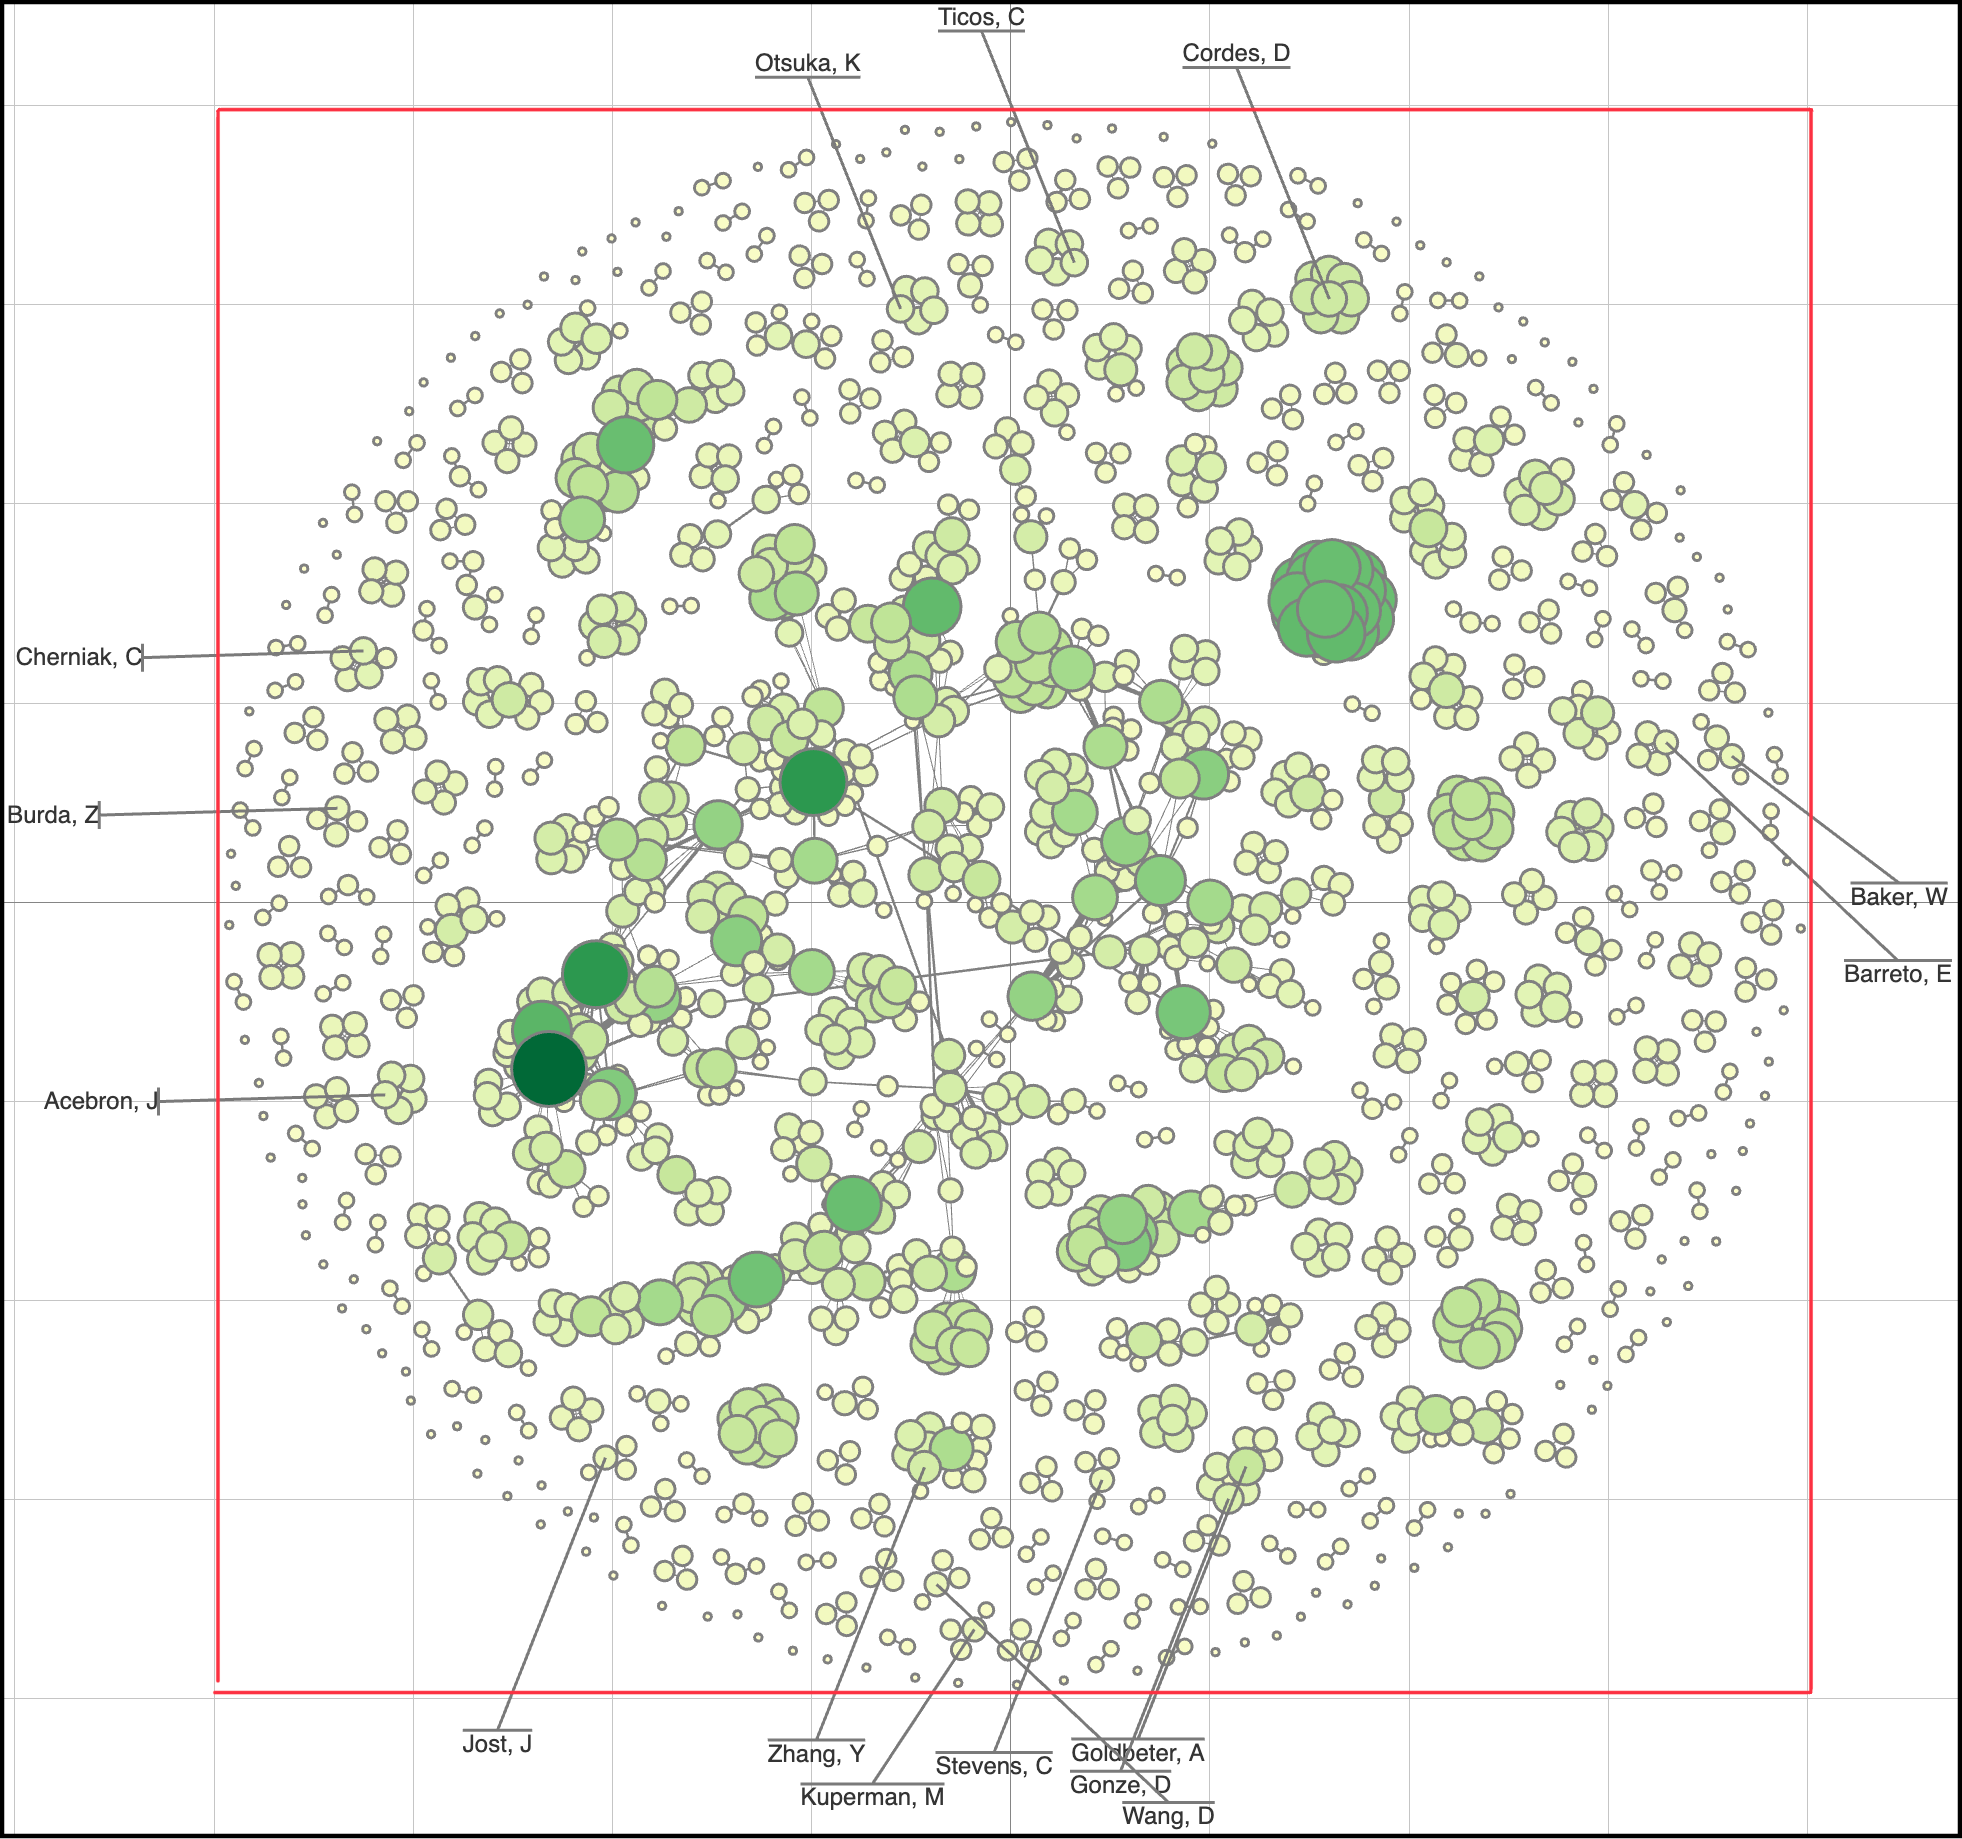
\includegraphics[scale=0.14]{../img/zoom}
    \caption{Zoom Mode aktiv. Außerdem zu sehen: Hilfslinie zwischen Knoten und Labels}
    \label{fig:zoom}
\end{figure}

\subsection{Performance Modes}
\label{subsec:perf}
    %Depending on visible amount, more or less complex procedures are used.

Performance Modes bilden ein Zusammenspiel aus der Anzahl der sichtbaren Knoten, also derjenigen, die in-bounds sind, und den
genutzten Labeling Verfahren. Allgemein gesagt: Je mehr Knoten sichtbar sind, desto weniger Verfahren werden genutzt -
und die genutzten Verfahren sind die einfacheren Verfahren.

Dies wird durch Grenzwerte realisiert (siehe \hyperref[subsec:consts]{Magic Constants}).
Die Grenzwerte (siehe \autoref{fig:perf_modes}) wurden vor allem durch manuelles Testen ermittelt.
Ziel war es das ein Labelingdurchlauf im Render-Loop möglichst unter $50$ ms bleibt.

\begin{figure}[H]
    \centering
    $$
    \begin{array}{c|c|l}
        \text{Minimum} & \text{Maximum} & \text{Verfahren}\\ \hline
        1 & 99 & \text{\hyperref[subsubsec:4pos]{4-Position-Model}, \hyperref[subsubsec:8pos]{8-Position-Model}, \hyperref[subsubsec:slider]{Slider-Model}, \hyperref[subsubsec:spiral]{Spiral-Model} }\\ \hline
        100 & 499 & \text{\hyperref[subsubsec:4pos]{4-Position-Model}, \hyperref[subsubsec:8pos]{8-Position-Model}, \hyperref[subsubsec:slider]{Slider-Model} }\\ \hline
        500 & 999 & \text{\hyperref[subsubsec:4pos]{4-Position-Model}, \hyperref[subsubsec:8pos]{8-Position-Model} }\\ \hline
        500 & \infty & \text{\hyperref[subsubsec:4pos]{4-Position-Model}}
    \end{array}
    $$
    \caption{Intervalle wie standardmäßig im Projekt festgelegt (siehe \hyperref[subsec:consts]{Magic Constants}) mit dazugehörigen Labeling Verfahren}
    \label{fig:perf_modes}
\end{figure}

Hier ist der Zweck, dass man bei sehr vielen sichtbaren Knoten durch das Labeling eine schnelle, grobe Orientierung bekommen kann.
Danach kann man via Zoom-In den gewünschten Bereich genauer explorieren, wofür dann auch ein aufwendiges und somit detailliertes Labeling wünschenswert wäre.
Da dann auch weniger Knoten zu sehen sind, was zu weniger Vergleichen führt, ist hier genug Zeit für solche komplizierten Berechnung.



\section{Visualization}
\label{sec:visualization}
Wenn ein potentielles Label nach Feststellen von Konfliktfreiheit zu einem tatsächlichen Label wird, so ist es für das Backend (wie in \hyperref[sec:conflict]{Conflict Detection und Bounds} beschrieben) relevant, dieses Label von nun an in der Konfliktermittlung zu berücksichtigen.
Für das Frontend gilt es dann, das Label an der gefundenen, freien Position zu zeichnen und animieren, sodass es für den Nutzer angenehmer anzuschauen ist.


\subsection{Drawing}
\label{subsec:draw}
    something with HTML canvas 

\subsection{Animation}
\label{subsec:animate}
    %3 modes depending on (visible now X visible before) (both not visible doesnt matter)
Die Animation finden immer dann statt, wenn sich der Sichtbarkeitszustand von Labels im Vergleich zur vorherigen Iteration des Render Loops ändert
oder es nach wie vor sichtbar ist, aber die Position des Labels sich geändert hat.
Das passiert, wenn in der neuen Iteration für ein anderes, wichtigeres Label diese Position gefunden wurde, dann im Nachhinein aber noch für das unwichtigere Label eine andere Position gefunden werden kann.
Wäre dies nicht der Fall, würde sich der Sichtbarkeitszustand zu nicht sichtbar ändern und das unwichtigere Label würde ausgeblendet werden (siehe \autoref{fig:animation}).

Hierfür wird die Klasse aus {Animatable.js} aus {iGraph.js} verwendet, die dort auch schon die Animation der Knoten händelt.
Somit werden Knoten und Labels durch dieselben Funktionen animiert.

\begin{figure}[H]
    \centering

   $$ \begin{array}{c|c|c}
                        & \text{sichtbar}_t & \text{nicht sichtbar}_t\\ \hline
         \text{sichtbar}_{t-1}   & \text{animate}   & \text{fade out} \\ \hline
        \text{nicht sichtbar}_{t-1} & \text{fade in}    & -
    \end{array}$$
    \caption{Zustände von Labelsichtbarkeit vor ($t-1$) und nach ($t$) dem Update der Positionen und die entsprechenden Animationsfunktionen}
    \label{fig:animation}
\end{figure}

\subsubsection{Fade In / Fade Out}
Diese Funktion verändern lediglich die Alpha-Werte, also die Transparenz, der Labels und ggf. der dazugehörigen Linien.
Für das Ausblenden werden sukzessive die Alpha-Werte dekrementiert, zum Einblenden werden sie sukzessive erhöht.

\subsubsection{Animate}
Da hier vor und nach dem Update das Label zu sehen ist, muss es verschoben werden.
Dabei kann es passieren, dass es kurzzeitig zu Überdeckung des von Labels und Knoten kommt.
In der finalen Position, nach der Animation, allerdings nicht mehr, da diese Position konfliktfrei ist.

Die Bewegungen bzw. die Animationen sind nicht rein linear, was das Labeling flüssiger, interaktiver und "lebendiger" erscheinen lässt, auch wenn es zusätzliche Berechnungen erfordert.
Diese können angestellt werden, da zuvor auf Effizienz geachtet wurde.



\section{Configuration}
\label{sec:configuration}

Die Konfiguration des Labeling kann über zwei Wege erfolgen:

Der erste ist der "User Mode" und erfolgt über ein minimales GUI, das bereits durch \texttt{iGraph.js} vorhanden war.
Neue Funktionalität wurden einfach in zusätzliche Buttons implementiert.

Der zweite Weg ist der "Author Mode". Es existiert ein File \texttt{consts.js}, in denen alle im Projekt
genutzten Magic Constants in einem Objekt zentral definiert sind und somit auch dort abgeändert werden könnten.
Die Standardeinstellungen sind allerdings getestet, auf \texttt{iGraph.js} zugeschnitten und haben sich über Monate etabliert.
Bei Änderung könnten ungewollte Konsequenzen und Bugs auftreten.

\subsection{GUI}
\label{subsec:gui}
    %small gui blending in with iGraph,
%toggle labels,
%in-/decrease fontsize and amount of labels shown.

Im Gegensatz zu Änderungen der Magic Constants ist das GUI sicher. Es beachtet festgelegte Minimal- und Maximalwerte
und sorgt dafür, dass diese nicht unterschritten bzw. überschritten werden (sofern die Standardwerte in \texttt{consts.js} verwendet werden).

Die durch das GUI zu ändernden Parameter sind:
\begin{itemize}
    \item Label anzeigen (Toggle)
    \item Anzahl angezeigte Labels erhöhen
    \item Anzahl angezeigte Labels reduzieren
    \item Schriftgröße erhöhen
    \item Schriftgröße reduzieren
\end{itemize}

Weiterhin gilt zu sagen, dass für die Anzahl der gezeigten Labels im \hyperref[subsec:zoom]{Zoom Mode} weniger Labels angezeigt werden als sonst.
Um hier filigraner einstellen zu können, erfolgt das De-/Inkrementieren der Anzahl der gezeigten Labels in Einserschritten.
Für den normalen Modus werden mehrere Labels auf einmal hinzugefügt bzw. gelöscht.

Um Berechnungen für große Graphen zu reduzieren sind geringe Labelanzahl und Schriftgröße eines der besten Werkzeuge, sollten allerdings vom User eingestellt werden können - daher ein GUI.


\subsection{Magic Constants}
\label{subsec:consts}
    %\texttt{consts.js} for all magic constants, easily configurable

Ursprünglich zum vereinfachten internen Testen und zur Strukturierung des Codes gedacht, ist
eine Sammlung der Magic Constants gegebenenfalls auch für externe Nutzer interessant. Viele Parameter, die über das GUI
nicht verstellt werden können sind hier konfigurierbar, beispielweise:
\begin{itemize}
    \item Schriftart und -farbe
    \item Interpolationsschritt für Kanten (siehe \hyperref[subsec:labeling_edges]{Kantenlabeling})
    \item Ineffizienzgrenzen der Teilregionen des Quadtree (siehe \hyperref[subsec:quadtree]{Quadtree}).
    \item Parameter der Spirale (siehe \hyperref[subsubsec:spiral]{Spiral-Model})
    \item Grenzwerte für die Performance Modes (siehe \autoref{fig:perf_modes})
\end{itemize}

Änderung an den Werten können immer dazu führen, dass das Programm gar nicht funktioniert oder zumindest nicht wie erwartet.
Für den Nutzung von gebräuchlichen Werten sollten allerdings maximal die Performance schlechter werden, Funktionalität aber erhalten bleiben.

Möglicherweise gibt es auch noch bessere Einstellungen hinsichtlich der Performance, die visuell gleichermaßen ansprechend sind wie die Standardeinstellungen.


\section{About the project}
\label{sec:about}

\subsection{Technical Details}
\label{subsec:technical}
    generator functions used, maps for fast access

\subsection{Known Bugs}
\label{subsec:bugs}
    %Flying Labels,
%Not Bug but consequence of implementation: Possible to have no labeling when everything is super dense

Beim Testen wurden die meisten Bugs behoben - ein selten auftretender Bug ist übrig geblieben:
"Flying Labels".

Manchmal kann es vorkommen, dass beim Fade Out von Labels diese von ihrer Position "wegfliegen" in eine Ecke des Bildschirms.
Dies fällt nur auf, wenn enorm viele Berechnungen stattfinden, also die Animationen langsamer sind.

Eine weitere ungünstige Konsequenz, die aus dem Fokus auf die Performance entstand:
Wenn alle sichtbaren Knoten als ineffizient markiert werden (und somit nicht gelabelt werden) und kein Zoom Mode möglich ist, z. B. wenn man Radar und Lens Funktion von \texttt{iGraph.js} nutzt,
dann wird gar nichts gelabelt.

Diese Situation sind aber praktisch unmöglich, man muss sie sehr gezielt erzwingen.

\subsection{Suggestions}
\label{subsec:suggest}
    %more conservative on animation side of things (keep positon as long as possible) => comes from implementation to always try to label most important stuff first
%better conflict detection with circle/bbox for Vertices
%better labeling for edges according to standards (leads to increased complixity in conflict detection for most cases)
%
%

Die Grundlage des Labeling wurde durch dieses Projekt erstellt. Auf der Seite der Performance wurden viele Techniken umgesetzt
und Möglichkeit genutzt um unnötige Berechnungen zu ersparen. Hinsicht der Visualisierung können aber vor allem noch Verbesserungen vorgenommen werden:

\subsubsection{Verbessertes Kantenlabeling}
Die Kantenlabels sollten ebenfalls nach kartografischen Standard gezeichnet werden. Das heißt, parallel zur entsprechenden Kante.
Dafür wären zum einen verbesserte Animationen nötig, um die Labels zu rotieren. Des Weiteren eine verbesserte Konfliktermittlung,
da dann nicht mehr garantiert werden kann, dass die Kantenlabels parallel zur $x$- und $y$-Achse sind.

\subsubsection{Verbesserte Repräsentation der Knoten als Kreis}
Das würde die Labelqualität verbessern, da die Labels noch näher an den Knoten wären und dementsprechend auch weniger Platz an jedem Knoten verschwenden (die Ecken der Bounding Box, die nicht Teil der Knotens sind).

Auch hier wäre eine verbesserte Konfliktermittlung, da die Knoten dann als Kreis statt als Bounding Box repräsentiert würden.
Zusammen mit dem ersten Verbesserungsvorschlag müsste man dann nicht Rechteckee parallel zur $x$- und $y$-Achse, sondern stattdessen beliebig orientierte Rechtecke und Kreise vergleichen, was wesentlich aufwendiger ist.

\subsubsection{Konservativere Animationen}
Zuweilen sind die Animationen sehr aktiv, was zu viel Unruhe im Labeling führt. Gegebenfalls sollte man eine Toleranzzeit einführen,
sodass sich Labels kurzzeitig überlappen dürfen, da viele Animationen durch minimale Überdeckungen während der Bewegungen entstehen.
Eine solche Toleranzzeit würde das Gesamtbild etwas statischer machen und einfach bei den \hyperref[subsec:consts]{Magic Constants} hinzugefügt werden.

\section*{Danksagung}
Ich möchte meinem Projektpartner Nico Trebbin für die Zusammenarbeit danken. Wir haben uns viel vorgenommen und viel davon umgesetzt.
Weiterhin danke ich Prof. Christian Tominski für das Semester, die Möglichkeit, auf seiner Codebasis aufzubauen und die Tipps, Anregungen und das Feedback während der Meetings.
Zu guter letzt möchte ich meiner Freundin Emily Fuhrmann für ihre Unterstützung in jeder Lage danken.

\bibliographystyle{plainnat} 
\bibliography{references.bib}

%\begin{landscape}
%    \begin{figure}
%        \centering
%        \includegraphics[width=\linewidth]{../03-labeling-nodes-and-edges-in-node-link-diagrams/doc/presentations/labeling algorithms/class_overview_4k.png}
%        \caption{Class Diagram}
%        \label{fig:classdiag}
%    \end{figure}
%\end{landscape}
%\includepdf[pages=-]{../03-labeling-nodes-and-edges-in-node-link-diagrams/doc/jsdoc/pdf/documentation2.pdf}

\end{document}
\endinput
